\documentclass{beamer}

\usetheme{Pittsburgh}
\usecolortheme{dove}

\usepackage[]{amsmath}
\usepackage{amssymb}
\usepackage{cmbright}
\usepackage{bm}

\newcommand{\RR}{\mathbb{R}}
\newcommand{\abs}[1]{|#1|}
\newcommand{\set}[1]{\{ #1 \}}
\newcommand{\defkey}{\textbf}

\title{A Stochastic Quasi-Newton Optimizer for \texttt{TensorFlow}}
\author[Chen, Kraemer]{%
Jason Chen\inst{1}, %
David Kraemer\inst{1}}

\institute[Stony Brook University]
{
  \inst{1}%
  CSE 592: Convex Optimization \\
  Stony Brook University
}

\date[2018]{May 1, 2018}


\begin{document}

\maketitle

\begin{frame}[t]{Problem overview}
  \begin{itemize}
    \item \texttt{TensorFlow} is an open source framework for building neural
      networks.
    \item It provides an interface for creating new \texttt{Optimizer}
      objects which perform different minimization algorithms.
    \item Typical existing implementations are first order descent
      algorithms, but it lacks\footnotemark any implementation of a BFGS-type
      algorithm.
  \end{itemize}
  \footnotetext[1]{See: \url{https://github.com/tensorflow/tensorflow/issues/446}}
\end{frame}

\begin{frame}[t]{Our contribution}
  \begin{itemize}
    \item We implemented stochastic dampened (Sd) L-BFGS in \texttt{TensorFlow} following the
      work of Wang, Ma, Goldfarb, and Liu (2017).
    \item The approach is based on the iteration step:
      \[
        x_{k+1} = x_k - \alpha_k H_k g_k,
      \]
    \item $\alpha_k$ is the step size,
    \item $H_k$ is the L-BFGS approximate Hessian,
    \item $g_k$ is a batch gradient defined as
      \begin{equation*}
        g_k = \frac{1}{m_k} \sum_{i=1}^{m_k} g(x_k, \xi_{k,i}),
      \end{equation*}
    \item $m_k$ is the batch size,
    \item $\xi_{k,i}$ is randomly sampled training data.
  \end{itemize}
\end{frame}

\begin{frame}[t]{Our contribution}
  \begin{itemize}
    \item The specific approach to approximating the Hessian differs from
      traditional L-BFGS implementations.
    \item Wang, et al showed that convergence (in expectation) is guaranteed by
      applying dampening at specific places in the approximation.
    \item Crucially, this holds even if the problem is \textbf{non-convex}.
    \item Their update, \texttt{SdLBFGS}, preserves the positive-definiteness of
      $H_k$ even in non-convex situations.
  \end{itemize}
\end{frame}

\begin{frame}[t]{Implementation}
  \begin{itemize}
    \item Implementing SdLBFGS proved challenging, and we discovered why it wasn't
      part of the library already!
    \item Following the advice from the discussion of 
      \href{https://github.com/tensorflow/tensorflow/issues/446}{Issue 446}, we
      implemented SdLBFGS as an \texttt{ExternalOptimizerInterface}.
    \item This allowed us to write \texttt{NumPy} code but ``plug in'' to
      \texttt{TensorFlow}.
  \end{itemize}
\end{frame}

\begin{frame}[t]{Results: sanity checks}
  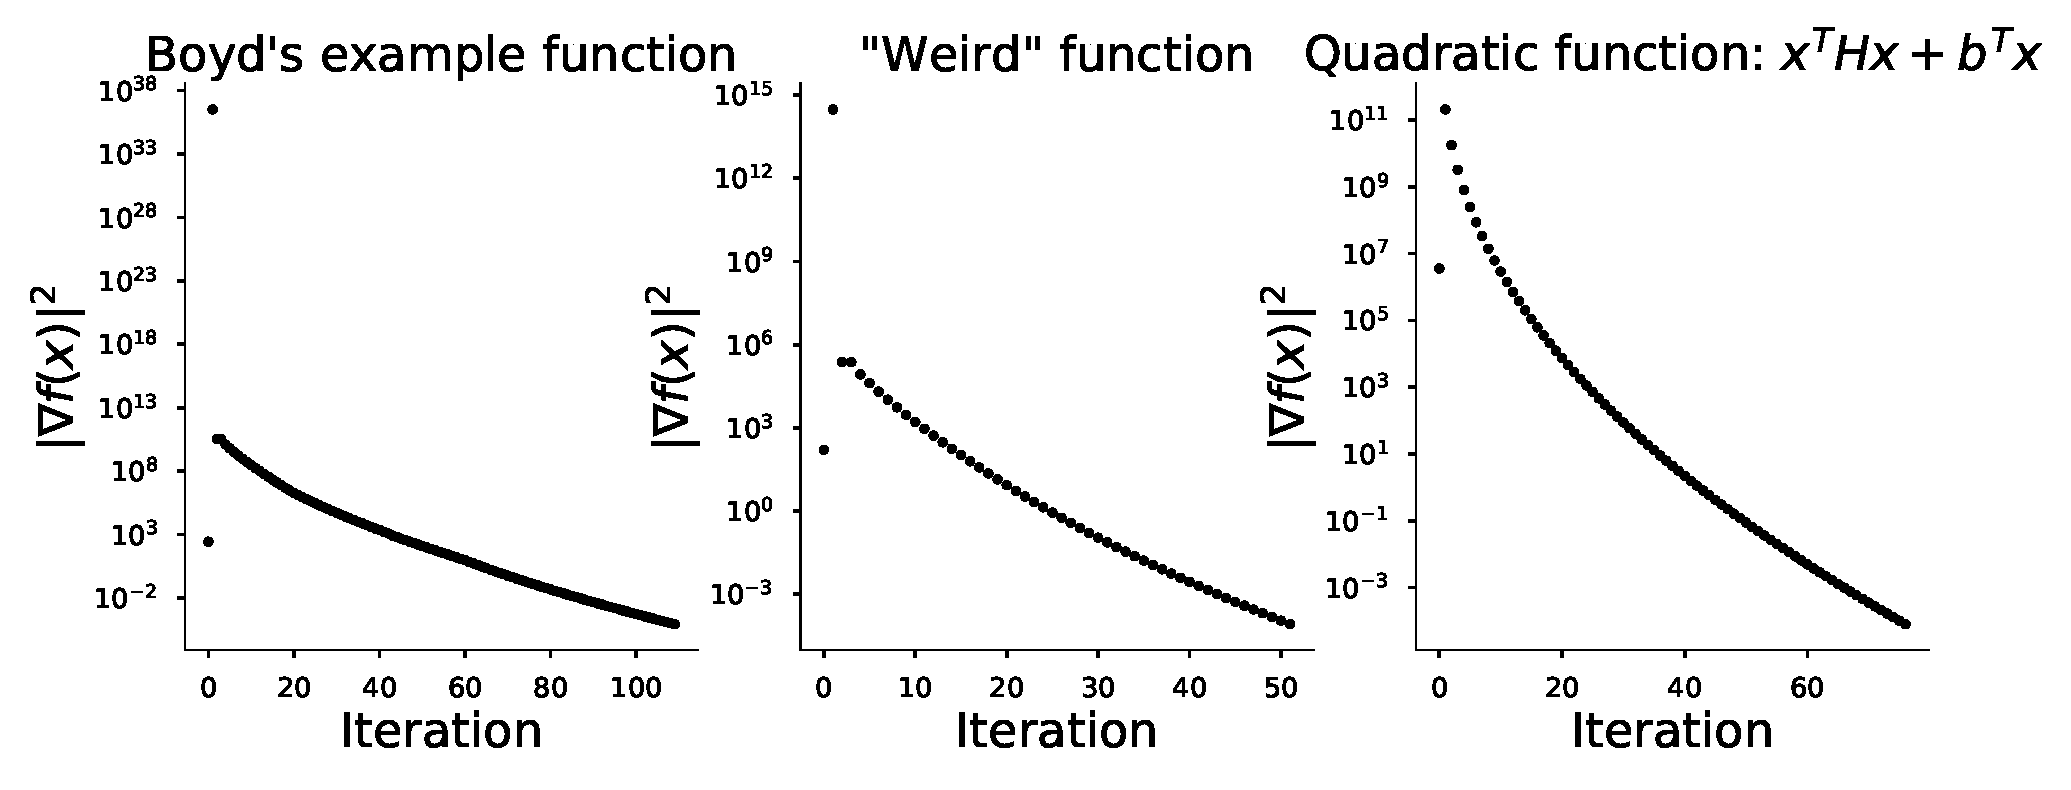
\includegraphics[width=\textwidth]{../plots/sanity_checks.eps} 
  \begin{itemize}
    \item Since our code is in \texttt{NumPy}, we could test it by running
      familiar homework functions.
    \item Here all gradients are deterministic.
  \end{itemize}
\end{frame}


\begin{frame}[t]{Results: Higgs dataset}
  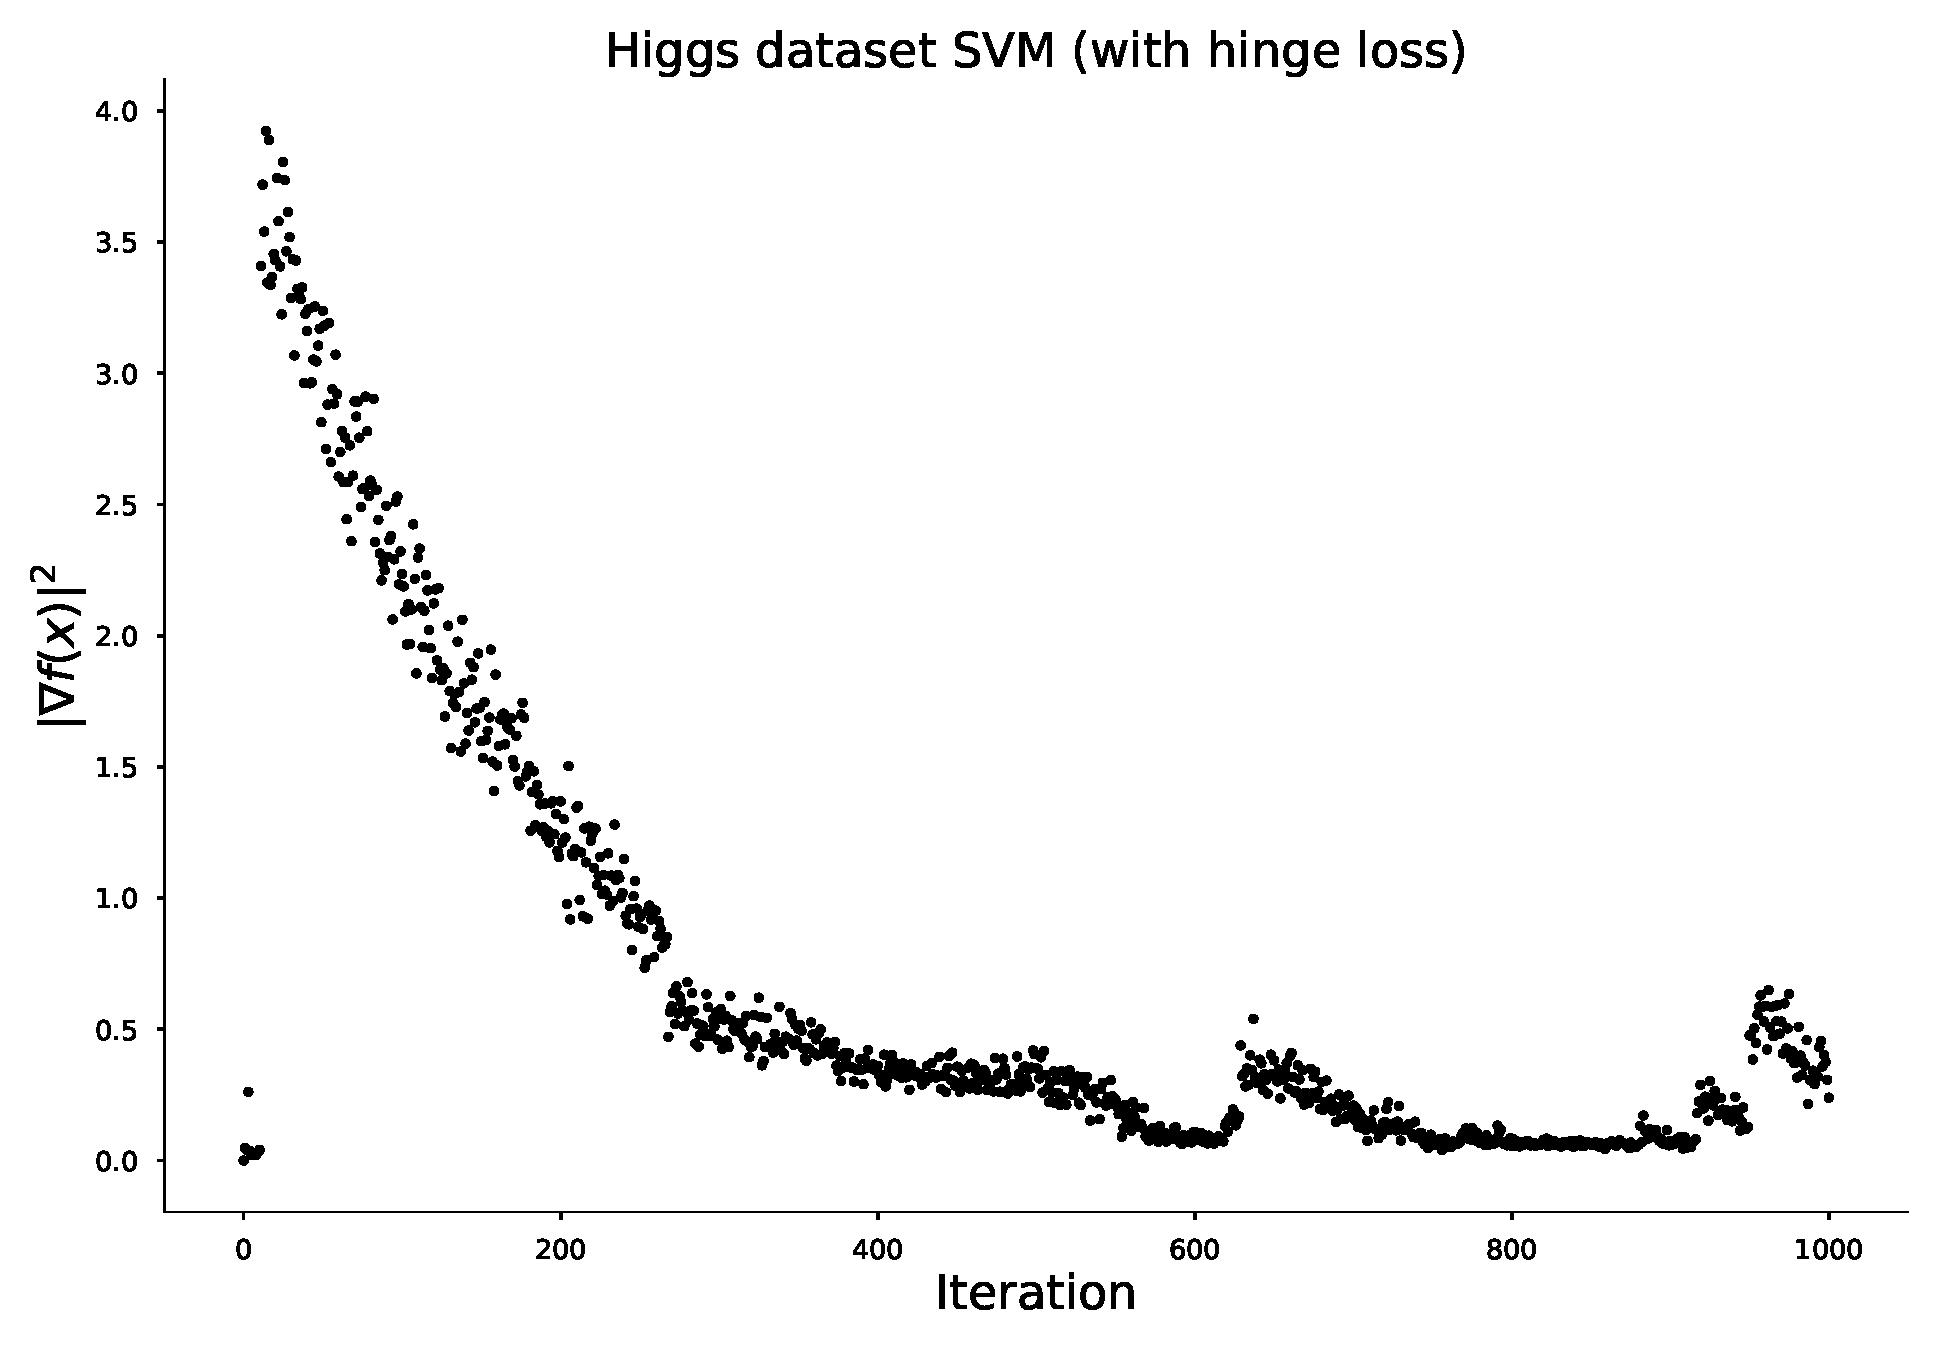
\includegraphics[width=\textwidth]{../plots/higgs_dataset.eps} 
\end{frame}

\begin{frame}
  
\end{frame}

\end{document}
